\newpage
\section{Wissenschaftlicher Teil}

\subsection{Analyse des Forschungsstandes}
Ziel der systematischen Literaturrecherche ist es eine Übersicht über den aktuellen Stand der Forschung zu erhalten und die Grundlage für die Konzeptionierung einer vollständigen, auf \ac{KI} basierten, Anwendung zu schaffen, welche Gastronomen dabei helfen soll, ihre Social Media Präsenz zu etablieren und durch Verwendung von generativen Machine Learning Algorithmen zu optimieren.
Durch die systematische Literaturrecherche sollen aktuelle Trends im Einsatz von \ac{KI} Technologien im Bereich der Gastronomie und des Social Media Marketings identifiziert werden, die anschließend in der Umsetzung der Projektarbeit berücksichtigt werden können.
Die Durchführung der systematischen Literaturrecherche basiert auf dem, nach vom Brocke et al. beschriebenen Vorgehen.\footcite{brocke2015standing}

Zur Bestimmung der eingesetzten Suchstrings, die für die Identifikation relevanter Literatur in den Literaturdatenbanken benötigt werden, wird zunächst die Problemstellung in einzelne Keywords zerlegt.
Die im Rahmen dieser Projektarbeit behandelte Problemstellung ist die Nutzung generativen KI, um die Social Media Präsenz von Gastronomen zu etablieren und zu optimieren.
Daraus resultieren folgende Keywords:

\begin{itemize}
    \item Generative Künstliche Intelligenz
    \item Social Media
    \item Marketing
\end{itemize}

Die Verwendung dieser Keywords bietet die Grundlage zur inhaltlichen Filterung der Literaturdatenbanken nach inhaltlichen relevanten Publikationen, die sich mit der untersuchten Problemstellung auseinandersetzen.
Zur Entwicklung eines Suchstrings werden die Keywords mit logischen Operatoren wie AND und OR kombiniert, um die Suche zu verfeinern und die Suchergebnisse zu reduzieren.
Daraus ergibt sich der folgende primäre Suchstring, welcher in den Literaturdatenbanken eingesetzt wird:

\begin{itemize}
    \item (``Generative AI'' OR ``Artificial Intelligence'' OR ``Generative Models'') AND (``AI-Driven Marketing'' OR ``Marketing Applications'' OR ``Content Creation'' OR ``Social Media Advertising'')
\end{itemize}

Die Durchführung der systematischen Literaturrecherche wird auf den folgenden online Portalen unter Verwendung des VPN-Zugangs der Hochschule durchgeführt:

\begin{itemize}
    \item EBSCO Discovery Service: \url{https://research.ebsco.com/c/mtvxwu/search}
    \item Elsevier ScienceDirect: \url{http://www.sciencedirect.com}
    \item Emerald Insight: \url{https://www.emeraldinsight.com}
    \item Google Scholar: \url{https://scholar.google.de}
    \item Springer Link: \url{https://link.springer.com}
\end{itemize}

Die Suchergebnisse werden nach Relevanz und Aktualität gefiltert, wobei bevorzugt Peer-Reviewed Paper betrachtet werden, die nicht älter als 10 Jahre sind.
Für die finale Auswahl einer Quelle erfolgt eine individuelle Bewertung anhand der Prüfung nach inhaltlicher Relevanz durch Untersuchung des Abstracts, sowie des Inhaltsverzeichnisses und zudem der Qualtität der Quelle durch ermittlung des H-Indexes des herausgebenden Journals.
Dokumentiert werden die Suchergebnisse in einer Literaturliste nach folgendem Schema:

\begin{tabular}{|l|l|l|l|l|l|}
\hline
Suchort & Suchalgorithmus & Anzahl Treffer & Auswahl & H-Index \\ \hline
\end{tabular}

Da die Suchergebnisse in den Literaturdatenbanken zu viele Treffer liefern und somit zu generisch sind, wird die Suche auf die letzten 10 Jahre beschränkt, um die Anzahl der Treffer zu reduzieren.
Zudem erfolgt eine Ergänzung der Keywords um die Begriffe:

\begin{itemize}
    \item Gastronomie
    \item Restaurant
    \item Food Service
\end{itemize}

um die Literaturrecherche auf den Erkenntnissen im Anwendungsbereich der Gastronomie einzuschränken.
Daraus resultiert eine Erweiterung des Suchstrings um den Begriff um den folgenden Begriff:

\begin{itemize}
    \item AND (``Gastronomy'' OR ``Restaurant'' OR ``Food Service'')
\end{itemize}

Abbildungen \ref{fig:Literaturtabelle_1} bis \ref{fig:Literaturtabelle_3} zeigen die Suchergebnisse der Literaturrecherche in den verschiedenen Literaturdatenbanken.

\begin{figure}[htbp]
    \centering
    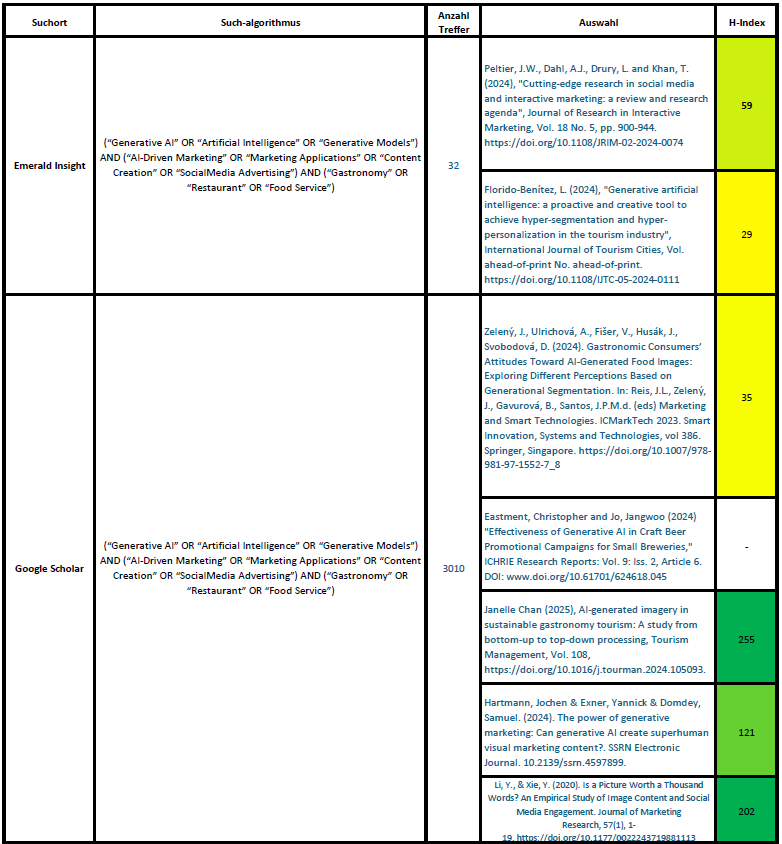
\includegraphics[width=\textwidth]{abbildungen/Literaturtabelle_1}
    \caption{Ergebnisse Literaturrecherche Teil 1}
    \label{fig:Literaturtabelle_1}
    \raggedright Quelle: Eigene Darstellung
\end{figure}

\begin{figure}[htbp]
    \centering
    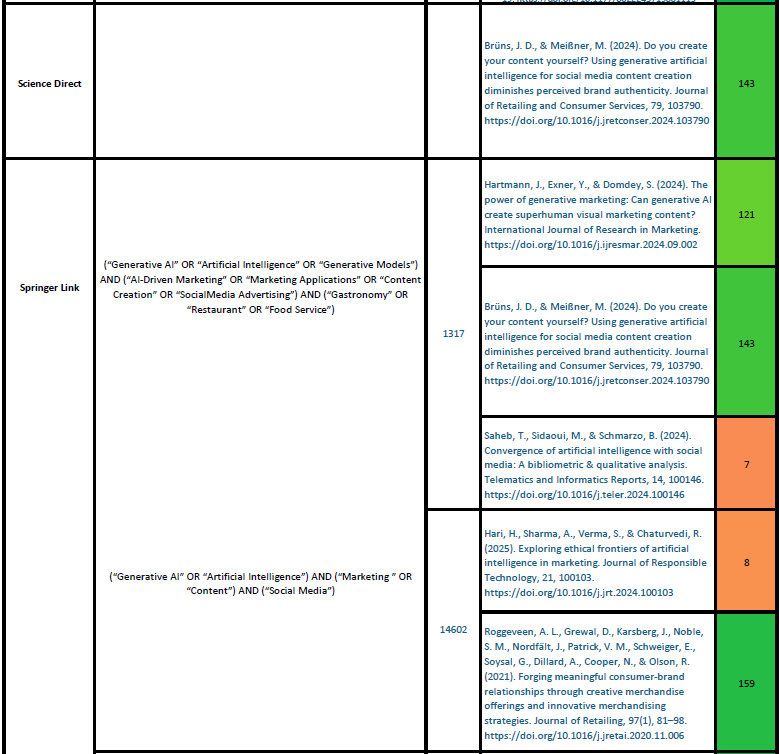
\includegraphics[width=\textwidth]{abbildungen/Literaturtabelle_2}
    \caption{Ergebnisse Literaturrecherche Teil 2}
    \label{fig:Literaturtabelle_2}
    \raggedright Quelle: Eigene Darstellung
\end{figure}

\begin{figure}[htbp]
    \centering
    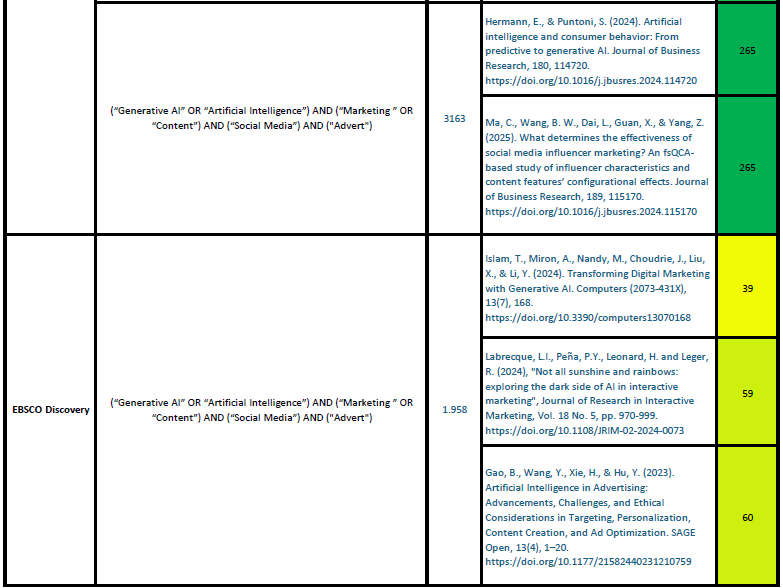
\includegraphics[width=\textwidth]{abbildungen/Literaturtabelle_3}
    \caption{Ergebnisse Literaturrecherche Teil 3}
    \label{fig:Literaturtabelle_3}
    \raggedright Quelle: Eigene Darstellung
\end{figure}

\subsection{Erläuterung des Anwendungsfalles}
Der Anwendungsfall beschreibt Gastronomen, die Unterstützung bei der Generierung von Social Media Inhalten benötigen, um die Attraktivität, die Aufmerksamkeit und den Umsatz ihres Lokals zu steigern.
Dabei wird eine \ac{KI} basierte Lösung entwickelt, welche Gastronomen zu einem Social Media Beitrag führt.
Die Lösung setzt dabei auf den Einsatz von generativen Machine Learning Algorithmen in Form von \ac{LLM}, um Bilder und Beiträge zu generieren.
Dabei kann der Gastronom selbst, mit Unterstützung, Einfluss auf die generierten Inhalte nehmen.
Die generierten Inhalte sollen, durch Unterstützung einer entsprechenden Benutzeroberfläche, zu einem vollständigen Social Media Post kombiniert werden.
Neben der Generierung der Social Media Posts soll der Gastronom zusätzlich über eine Kalenderansicht verfügen, um den Status aktueller und zukünftiger Social Media Kampagnen einzusehen.
Damit eine Lösung adäquat und tragend entwickelt werden kann, bedarf es einer Markt- und Wettbewerbsanalyse, um eine strategische Auswahl einer Social Media Plattform und ein Konzept zur Monetarisierung der entwickelten Lösung entwickeln zu können.
Hierbei soll sich der erste Anwendungsfall vorerst auf nur eine einzige Social Media Plattform konzentrieren.

\subsection{Markt- und Wettbewerbsanalyse}
Die Markt- und Wettbewerbsanalyse ist ein Vorgehen, welches eingesetzt wird, um eine Übersicht über die Möglichkeiten am Markt und die potenziellen Wettbewerber zu erlangen.
Dabei bietet der Markt, bezogen auf den Anwendungsfall, vielversprechende Möglichkeiten im Einsatz von generativer \ac{KI} im Social Media Marketing Bereich der \ac{KMU}.
So geht aus einer Datenerhebung durch Statista hervor, dass das Wachstum von \ac{KI} basierten Lösungen im Marketingbereich bis zum Jahr 2028 einen Umsatz von bis zu 107.5 Mrd. USD erreichen kann.\footcite{statista_ai_marketing_europe}

Ebenfalls zeigt eine Studie von McKinsey, dass der Einsatz von Technologien, wie generative \ac{KI}, eine erhebliche Steigerung der Produktivität zufolge haben kann.\footcite{mckinsey_genai_marketing}

In der Gastronomiebranche wird die Wichtigkeit und potenzielle Wachstumsfaktoren durch Social Media Marketing besonders dadurch deutlich, dass ca. 37 Prozent\footcite{apicbase_gastro_fakten} der Kunden die Social Media Seiten der Gastronomien besuchen, bevor diese sich für einen Besuch des Lokals entscheiden.
Generell informieren sich vor einem Restaurantbesuch ca. 84 Prozent\footcite{g_wie_gastro_trends_2024} der Kunden vorab online.
Ebenfalls lässt sich laut einer Erhebung von Statista beobachten, dass die Interaktion zwischen Gastronomen und Gästen, seit der Popularität von Social Media, eine Veränderung erfahren hat.\footcite{statista_social_media_gastgewerbe}

Unternehmen wie Killian, MARA und Jasper.ai haben sich bereits auf dem Markt etabliert und bieten KI basierte Lösungen im Bereich des Social Media Marketings an.

Killian ist eine speziell auf die Hotel- und Restaurantbranche ausgerichtete Lösung, die diverse Funktionalitäten anbietet, wie beispielsweise Bewertungsmanagement, Content Management, E-Mail-Marketing, Public Realtions, und Social Media.\footcite{kilian_ai_produkt}
Dabei setzt Killian auf generative \ac{KI} und setzt hierfür Modelle, wie das GPT4 Modell von OpenAI, ein.
Klare Vorteile dieser Lösung sind einerseits der Umfang, andererseits der Fokus auf die Gastronomie- und Hotelbranche im Einsatz von generativer \ac{KI}.
Als wesentlichen Nachteil aus ökonomischen Aspekten des Gastronoms ist das Bezahlmodell des Produktes, in Form einer 14-Tägigen Testversion mit anschließendem Zwang zum Kauf einer Premiumvariante zu erwähnen.\footcite{kilian_ai_preise}
Ein weiterer Nachteil ergibt sich aus der mangelnden End-to-End-Funktionalität, da keine direkte Möglichkeit besteht, aus der Applikation auf Social Media zu publizieren.\footcite{kilian_ai_funktionen}

MARA positioniert sich als Bewertungsmanagementlösung, unter Einsatz von generativer \ac{KI}, als weiterer Wettbewerber.
Dabei liegt der Fokus dieser Lösung primär auf der Bearbeitung von Bewertungen, wie zum Beispiel Google Bewertungen und Kommentaren auf Social Media Plattformen, jedoch nicht auf der Generation branchenspezifischer Inhalte in der Gastronomiebranche.
Ein Nachteil des Produktes Mara ist die fehlende Funktionalität zur Generierung von Bildern.\footcite{mara_solutions_features}
Inhaltlich hebt sich das Produkt somit von der Lösung ab, die im Rahmen dieser Projektarbeit entwickelt wird und ist somit kein direkter Wettbewerber.

Jasper.ai, als dritter Wettbewerber, setzt auf ein generisches KI-Tool für die Generierung von Marketing-Content.
Sowohl die Generierung von Texten, als auch die Generierung von Bildern wird durch den Einsatz von generativer \ac{KI} ermöglicht.
Hierbei ist zu erwähnen, dass Jasper.ai nicht branchenspezifisch ist und somit keine individuellen Lösungen für die Gastronomiebranche anbietet.\footcite{jasper_ai_product_marketers}

Alle der untersuchten Wettbewerberprodukte erfordern eine gewisse Vorerfahrung im Umgang mit KI-Technologien, um die Lösungen effektiv einsetzen zu können.

\subsection{Kundenanalyse}
Für die Festlegung des typischen Kunden dieser Lösung wird in erster Linie die Zielgruppe definiert und die Erwartungen der Kunden, an diese Applikation, evaluiert.

Die primäre Zielgruppe sind \ac{KMU} Gastronomiebetriebe, beispielsweise kleine lokale Pizzalieferdienste bis hin zu mittelgroßen Restaurants, da diese die Hauptkunden der DISH-Consulting GmBH sind.
Die daraus entstehende Problematik ist, dass keine, der für die Entwicklung von umfangreichen Marketingstrategien notwendigen, Kompetenzen im Betrieb vorhanden sind, aufgrund mangelndem Budget für Marketingaktivitäten.\footcite{restroworks2024}
Zu einem effektiven Marketingkonzept gehört ebenfalls der Gebrauch von Social-Media-Maßnahmen.

Dementsprechend könnten Erwartungen von zukünftigen Kunden dieser konzeptionierten Applikation sein, dass exakt die oben genannten Problematiken kosteneffizient aufgegriffen werden.
Genauer gesagt antizipieren sich die Erwartungen dahingehend, dass hochwertiger Social-Media-Content generiert werden soll, der als Teil einer Marketingmaßnahme die Bekanntheit des Gastronomiebetriebs steigern soll.
Eine effektive Marketingkampagne dient der Generierung von Kunden und Markenreichweite und hat somit höhere Umsätze aufgrund steigender Verkaufszahlen für den Betrieb zufolge.
Eine weitere Erwartung an die Generierung des hochwertigen individuellen Social-Media-Contents ist die Bereitstellung eine benutzerfreundlichen Anwendung, die eine einfache und intuitive Nutzung der verfügbaren Funktionalitäten auf Anwendungsebene ermöglicht.

Die beschriebenen Erwartungen lassen sich in die Sammelbegriffe Umsatzoptimierung, Zeiteffizienz, Kostenersparnis und Prozessoptimierung gruppieren.

\subsection{SWOT-Analyse}
Die Durchführung einer SWOT-Analyse soll die Stärken, Schwächen, Chancen, als auch Risiken für die Nutzung der Anwendung aufzeigen, um eine Übersicht der Möglichkeiten zu generieren.
Eine Stärke der in dieser Thesis konzeptionierten Anwendung soll durch die Branchenspezialisierung auf den Gastronomiesektor erfolgen.
Eine weitere Stärke soll das vollständige Design einer End-to-End-Lösung darstellen, welche den Gastronom von der Idee, bis hin zu der finalen Veröffentlichung eines Social Media Beitrages untersützt wird.
Die dritte und gleichzeitig wichtigste Stärke soll durch eine sehr hohe Benutzerfreundlichkeit, zur Reduzierung jeglicher Einstiegshürden für technisch unerfahrene Nutzer, dargestellt werden.

Die signifikanten Schwächen dieses Tools sind einerseits die technologische Abhängigkeit von der Qualität und Leistungsfähigkeit der Large Language Modelle, andererseits die etablierte Konkurrenz, welche bereits eine starke Marktpräsenz etabliert haben.

Die Chancen, die durch den Einsatz dieses Tools entstehen, sind zum Einem die wachsende Nachfrage nach Automatisierung, durch steigende Akzeptanz von KI-Tools in der Gastronomie.
Zum anderen das Potenzial zur Expansion auf weitere Branchen, wie beispielsweise die Hotellerie und zuletzt die Möglichkeit, einzigartige Inhalte zu erstellen, die individuell auf die Bedürfnisse des Kundens zugeschnitten sind.

Mögliche Risiken durch den Einsatz dieses Tools sind Datenschutzbedenken.
Durch Verarbeitung von sensiblen Daten, wie bspw. dem Kalender, könnten Datenschutzverletzungen entstehen.
Ein weiteres bestehendes Risiko, ist das volatile Umfeld, in dem die Anwendung eingesetzt wird, da der Markt, in der Gastronomie und KI, sich stetig weiterentwickelt, sodass ggf. schnelle Anpassungen der Lösung erforderlich sind.

\begin{figure}[htbp]
    \centering
    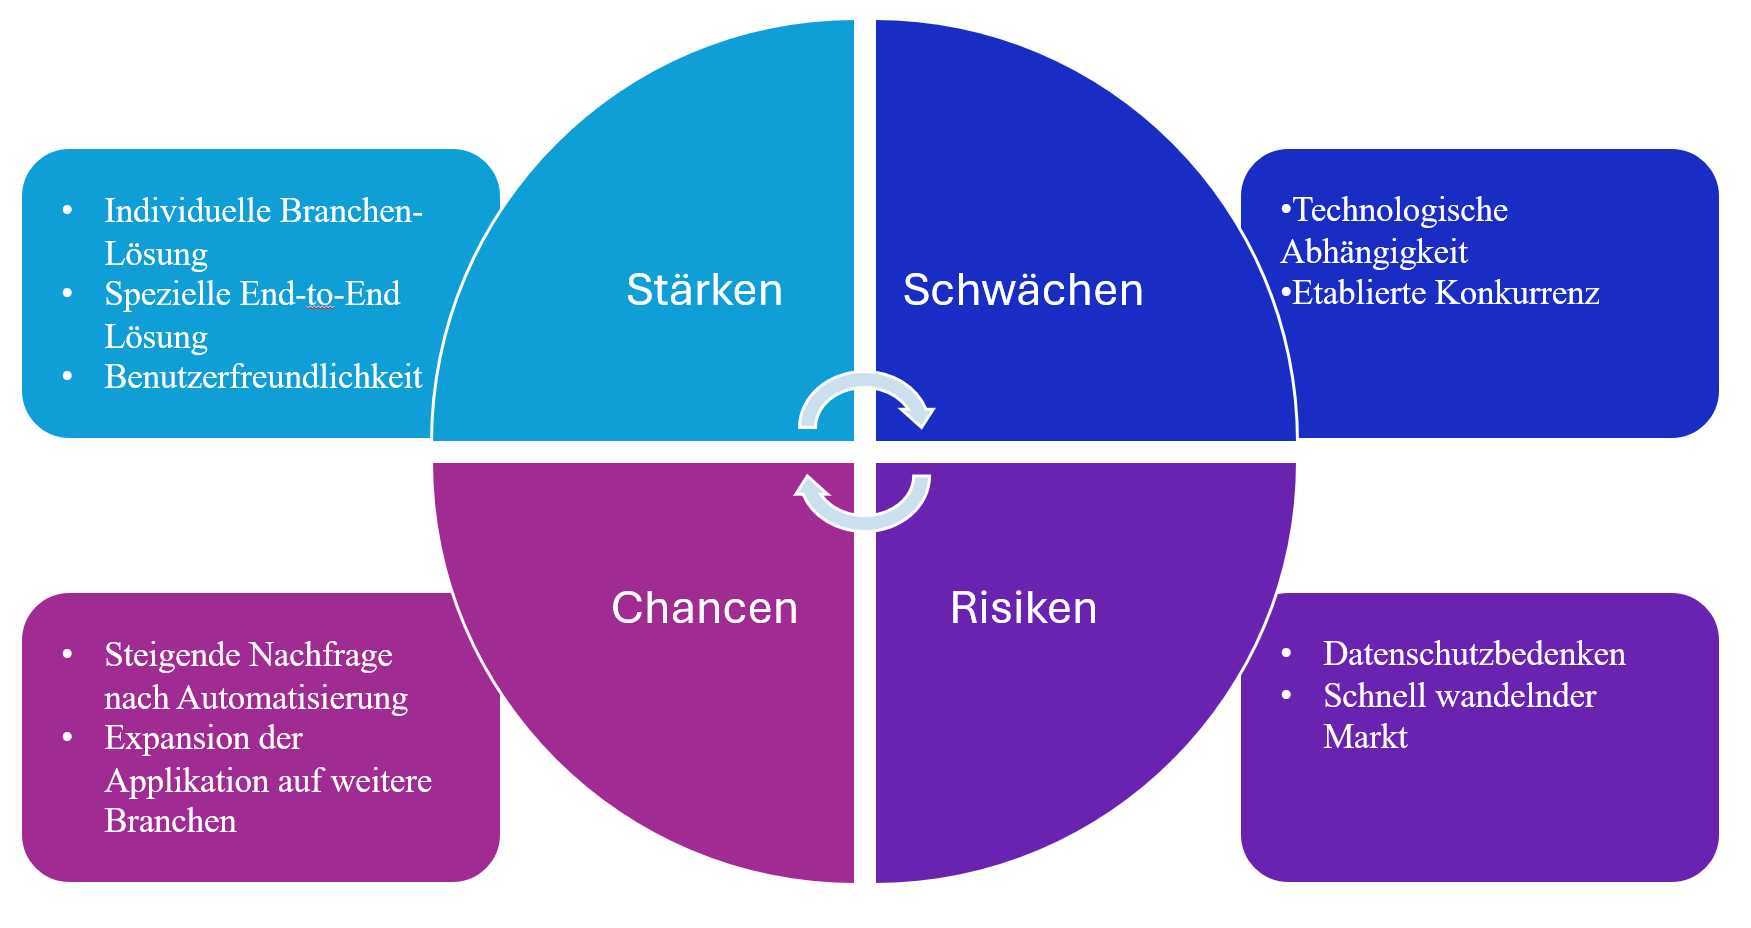
\includegraphics[width=0.8\textwidth]{abbildungen/SWOT}
    \caption{SWOT-Analyse}
    \label{fig:SWOT-Analyse}
    \raggedright Quelle: Eigene Darstellung
\end{figure}

\subsection{Strategische Auswahl der Social Media Plattformen}
Ergänzend zur Markt- und Wettbewerbsanalyse bedarf es ebenfalls an der strategischen Auswahl einer geeigneten Social Media Plattform.
In der ersten Iteration der Entwicklung einer KI-basierten Social-Media-Kampagnenlösung ist es sinnvoll, sich auf eine einzige Plattform zu begrenzen.
Einerseits zeigen alle verfügbaren Social Media Plattformen Ähnlichkeiten im Aufbau und der Struktur zueinander auf, andrerseits funktioniert Plattform nach seinen eigenen .
Zur Auswahl stehen laut dem „Digital 2024 Global Overview Report“ von Hootsuite eine Vielzahl an Social Media Plattformen.
Gemessen an den aktiven Benutzern auf den Plattformen bilden die Social Media Plattformen Facebook (ca. 3.05Mrd.), YouTube (ca. 2.49Mrd.), WhatsApp (ca. 2.00Mrd.), Instagram (2.00Mrd.) und TikTok (ca. 1.56Mrd.) die fünf Plattformen mit den höchten Nutzungsraten.\footcite{hootsuite_digital_2024_page_232}
Das Unternehmen Meta betreibt hierbei drei der fünf genannten Plattformen (Facebook, WhatsApp und Instagram).
Die Social Media Plattformen YouTube und TikTok sind Plattformen, die primär Videos in Form von Lang- und Kurzformaten anbieten.
Das bedeutet, dass sämtliche Beiträge, die dort durch Benutzer erstellt werden, ausschließlich Videobeiträge sind.
Die Plattform WhatsApp ist in erster Linie ein Messenger-Dienst, der für Privatnachrichten und Anrufe zwischen mehreren Personen genutzt werden kann.
Dies funktioniert jedoch nur dann, wenn die Telefonnummern den Personen bekannt sind, im Gegensatz zu den anderen Social Media Plattformen, die auf Nutzernamen setzen.
Instagram, als auch Facebook setzen auf ein Konzept, bei dem jeder Benutzer öffentliche, als auch private Bild-, Text-, Videobeiträge veröffentlichen kann, die entweder der gesamten Nutzerschaft der Plattform angezeigt werden, oder nur den befugten Benutzern auf der Freundesliste.
Ebenfalls verfügen die Plattformen über einen Messenger-Dienst, ähnlich wie bei WhatsApp.

Aus dem „Digital 2024 Global Overview Report“ von Hootsuite geht hervor, dass Instagram, trotz der geringeren Nutzerzahl im Vergleich zu Facebook, WhatsApp und YouTube, dennoch die beliebteste bei Nutzern zwischen dem Alter 16 und 64 ist, wie aus dem Report hervorgeht.\footcite{hootsuite_digital_2024_page_236}
Ebenfalls geht aus diesem Report hervor, dass ca. 63 Prozent der Nutzer der Plattform Instagram im Alter zwischen 16 und 64, diese Plattform nutzen, um Unternehmen zu suchen und investigieren.\footcite{hootsuite_digital_2024_page_250}
Dementsprechend ist die Entwicklung der KI-basierten Social-Media-Kampagnenlösung auf die Social Media Plattform Instagram ausgerichtet.

\subsection{Strategie zur Monetarisierung des Anwendungsfalles}
Zu einer vollständigen Betrachtung des Anwendungsfalles gehört ebenfalls auch die Entwicklung eines Konzeptes zur Monetarisierung des Prototypen.
Im Fokus stehen einerseits die Generierung von Social Media Posts über die Benutzeroberfläche und andererseits der Kalender, welcher zur Übersicht und Planung weiter Social Media Posts genutzt werden kann.
Ein Ansatz dieses Produkt zu vermarkten wäre die Monetarisierung durch den Vertrieb einer ausschließlichen Premiumvariante dieser Lösung.
Die ausschließliche Premiumvariante würde sich durch drei Begründungen ergeben.
Zum einem wäre diese KI-basierten Social-Media-Lösung als Erweiterung der bestehenden Lösungsplattform der Dish Consulting GmbH zu betrachten, bei der sich bestehende Kunden diesen Service dazubuchen könnten.
Zum anderem würde sich die ausschließliche Premiumvariante dahingehend begründen, dass die bestehenden Marktteilnehmer, wie Killian und Jasper, auf ausschließliche Premiumvarianten setzen.
Somit würde sich diese Lösung nur dem bestehenden Marktumfeld in der Monetarisierungsstrategie einfügen.
Zuletzt begründet sich die Wahl der Premiumvariante dahingehend, dass bestehende Kosten unbedingt gedeckt werden müssen und bei anderen Monetarisierungsmodellen, wie z. B. der Freemium-Variante dies nicht zwangsweise gegeben ist.
Die Freemium-Variante baut auf dem grundlegenden Gedanken, dass ein Teil der Lösung kostenfrei ist und bestimmte Funktionalitäten oder eine uneingeschränkte Nutzung der Applikation entsprechend bezahlt werden muss.
Die Problematik, die sich hierbei ergeben kann, dass die Kunden eben entsprechend nicht auf die Premiumvariante hochstufen und sich damit die Kosten nicht vollständig decken.
Diese grundlegende Problematik geht aus einigen Studien hervor, dass der Nutzen und die Nutzerbasis der Lösung groß genug sein muss, dass eine hohe Umwandlungsrate zur Premiumvariante gegeben ist.
In spezielleren Branchen, wie z. B. die Gastronomie im \ac{KMU} Segment könnte die hohe Nutzerbasis nicht gegeben sein und damit könnte auch die Umwandlungsrate kleiner ausfallen.\footcite{kumar2014freemium}
Eine weitere Problematik, die sich aus dem Freemium-Modell ergeben könnte ist die fehlende Evidenz über den Nutzen der Premiumfunktionen der Lösung, sodass sich überhaupt keine Notwendigkeit (aus sich des Kunden) auftut auf die Premiumvariante hochzustufen.
Dieser Umstand würde ebenfalls die Umwandlungsrate zur Hochstufung des Services negativ beeinträchtigen.\footcite{kim2018perceived}

Durch das Anbieten von verschiedenen Abonnement-Modellen, wie beispielsweise einem Monats- oder Jahresabo, kann der Kunde die für ihn passende Variante auswählen.
Neben der offensichtlichen Monetarisierung der entwickelten Lösung, könnte man durch Einwilligungserklärungen der Gastronomen deren eingegebenen Daten verarbeiten, sodass ein weiteres Konzept der Monetarisierung entsteht.
Die erhobenen Daten, die bspw. durch die Kalenderfunktionalitäten entstehen, wie „Wann plane ich einen Beitrag?“, oder „Wie viele Kampagnen laufen aktuell?“, liefern wertvolle Informationen, die direkt oder indirekt monetarisiert werden können, durch Verkauf der Daten, oder der Entwicklung von Machine Learning ALgorithmen auf Basis der Daten, wie z.B. „Wann ist der beste Zeitpunkt für eine Kampagne?“, welche anschließend gewinnbringend eingesetzt werden können.
Genauso ist die Erhebung der eingegebenen Prompts der Gastronomen ein wichtiger Aspekt zur Monetarisierung und Konzeptionierung weiterer Funktionalitäten dieser Lösung.

\subsection{Evaluation einzusetzender Technologien}

\subsection{Evaluation und Auswahl generativer Machine Learning Modelle} %Todo: Kapitel strukturieren
Die in einem späteren Kapitel thematisierten Eigenschaften von Social Media Posts beschreiben die wichtigsten Charakteristiken, um die Aufmerksamkeit und Interaktionsrate von Social Media Nutzern zu maximieren und somit potenzielle Leads zu einer Kaufentscheidung zu bringen.
Hierbei ist zu beachten, dass der Social-Media-Content ideal auf die jeweilige Social Media Plattform abgestimmt ist und die Zielgruppe emotional anspricht, damit sich dieser besser in Erinnerung bleibt.
Zudem sollte der Social-Media-Content eine klare und konsistente Botschaft transportieren.

Des Weiteren sollten veröffentliche Inhalte einen hochwertigen Eindruck vermitteln und sowohl farblich als auch typografisch mit der Markenidentität übereinstimmen.
Eine zentrale Aufgabe im Bereich des Social Media Marketings ist somit die Erstellung und Veröffentlichung von hochwertigem, zielgruppengerichteten und aussagekräftigen Content, der Zielgruppen zu einer Kaufentscheidung animiert, oder den Wiedererkennungswert eines Produktes oder einer Marke steigert.

Die Generierung von Social-Media-Content durch den Einsatz von generativen Machine Learning Modellen dient als kostengünstige Alternative gegenüber konventionellen Methoden, wie der Verwendung von kommerziellen Bildern oder der Beauftragung von Grafikdesignern.\footcite[1-2]{hartmann2024power}
Während ein professionell erstelltes, kommerzielles Bild durchschnittlich 5 bis 10 Euro kostet, kann die Generierung von Bildern durch den Einsatz von generativen Machine Learning Modellen wie beispielsweise OpenAI´s DALLE-E 3 bereits ab 0,038 Euro pro Bild erfolgen.\footcite{betker2023improving}
Statistiken zufolge wird das wirtschaftliche Potenzial von KI im Bereich des Marketings auf auf 463 Milliarden US-Dollar geschätzt. \footcite{chui2023economic}

Diese Entwicklung hat dazu geführt, dass heutige state-of-the-art KI-Modelle dazu Fähig sind, Social Media Content jeglicher Art, egal ob in Bild-, Text-, oder Videoform zu erzeugen, welcher sich ohne Weiteres nicht von menschlich generierten Content unterscheiden lässt und den Eindruck von hochwertig generierten Werbeinhalten vermittelt.\footcite[1]{hartmann2024power}
Auf eine Vielzahl dieser äußerst leistungsfähigen Modelle kann über das Internet kostenlos zugegriffen werden.
Machine Learning Plattformen wie Hugging Face bieten die Möglichkeit, vortrainierte Machine Learning Modelle mit unterschiedlichen Modellzielen, wie beispielsweise Text-to-Image, Text-to-Text, Text-to-Voice, kostenlos herunterzuladen und auf eigenen Hardware Ressourcen zu verwenden.\footcite{huggingface}
Die Auswahl eines geeigneten Machine Learning Modells ist, neben der Erschaffung eines optimalen prompts zur Nutzung des Modells, von zentraler Bedeutung für die Qualität des Ergebnisses, da sich die generativen Modelle in ihren Hyperparametern und den angewandten Trainingsprozessen voneinander unterscheiden. \footcite[S. 9 ff.]{betker2023improving}

Die Auswahl der im Rahmen dieser Projektarbeit eingesetzten generativen Machine Learning Modelle zur Generierung von Social Media Content basiert auf den folgenden Faktoren:

\begin{itemize}
    \item Modellziel: Die Art der Aufgabe, die durch das Machine Learning Modell bearbeitet werden kann wie z.B. Übersetzungen, Texterzeugung, Bilderzeugung, Bildbeschreibung, Objekterkennung.
    \item Qualität: Die Qualität der generierten Inhalte in Hinblick auf Kreativität, Realismus, Kohärenz und Nutzbarkeit.
    \item Leistung: Dauer für die Generierung von Inhalten sowie Konsistenz in den Ergebnissen.
    \item Integration: Integrationsmöglichkeiten des Modells mit weiteren Systemen.
    \item Größe: Umfang des Modells, sowie der benötigten Rechenanforderungen zur Verwendung des Modells.
\end{itemize}

Unter der Annahme, dass ein Engagement fördernder Social Media Post aus einer grafischen Komponente besteht, welche die Aufmerksamkeit des Nutzers initial erregt und einem beschreibenden Text, um den Nutzer mit zusätzlichen Informationen über die präsentierten Inhalte zu versorgen, lässt sich der in Abbildung \ref{fig:process_content_generation} beschriebene Prozess für die KI-basierte Generierung von Social Media Content definieren.
\begin{figure}[htbp]
    \centering
    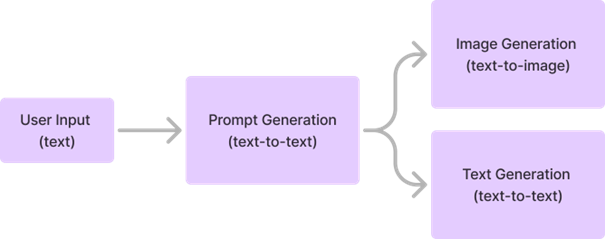
\includegraphics[width=\textwidth]{abbildungen/Process_image_generation}
    \caption{Prozess zur KI gestützten Social Media Content Generierung}
    \label{fig:process_content_generation}
    \raggedright Quelle: Eigene Darstellung
\end{figure}

Der Anwender startet den Prozess mit der Angabe von Informationen über das gewünschte Produkt, für welches der Social Media Content generiert werden soll.
Im ersten Verarbeitungsschritt wird diese Informationen von einem Text-to-Text Machine Learning Modell verarbeitet, um daraus einen Prompt zu generieren, welcher als Basis dient, um die finalen Social Media Inhalte zu generieren.
Entscheidend ist hierbei die Erweiterung der Produktangaben um stilistische Anweisungen und werbespezifischen Details, um ein möglichst engagement förderndes Ergebnis zu erzielen.
Der finalisierte Prompt, welcher als Basis für die Generierung von Bild und Text dient, wird anschließend einerseits ein weiteres Mal in ein Text-to-Text Machine Learning Modell übergeben, um daraus eine aussagekräftige Social Media Beschreibung in Textform zu generieren und andererseits in ein Text-to-Image Modell, um ein ansprechendes Bild zu generieren, welches für die Bewerbung des gewünschten Produktes geeignet ist.
Zur Auswahl eines geeigneten Text-to-Image Modells wurden die beschriebenen Bewertungskriterien herangezogen um eine einheitliche Vergleichsbasis zu schaffen.
Die bewerteten Modelle basieren hierbei auf den populärsten Modellen der Machine Learning Plattform Hugging Faces.\footcite{huggingface_models}

Verglichen wurden unter anderem bekannte Modelle von etablierten Unternehmen, wie die Stable-Diffusion Modelle der Firma Stability-AI oder die FLUX Modelle der Firma Black Forest Labs.\footcite{stabilityai,blackforestlabs}
Um die Leistungsfähigkeit der Modelle zu vergleichen und anschließend eine finale Auswahl je Modellziel treffen zu können, wurde ein identischer Prompt mit der Anweisung zur Generierung eines Döner Kebabs den verschiedenen Modellen übergeben.
Anschließend wurde die benötigte Zeit zur Generierung des Outputs, sowie der Output selbst miteinander verglichen.
\clearpage
\begin{figure}[htbp]
    \centering
    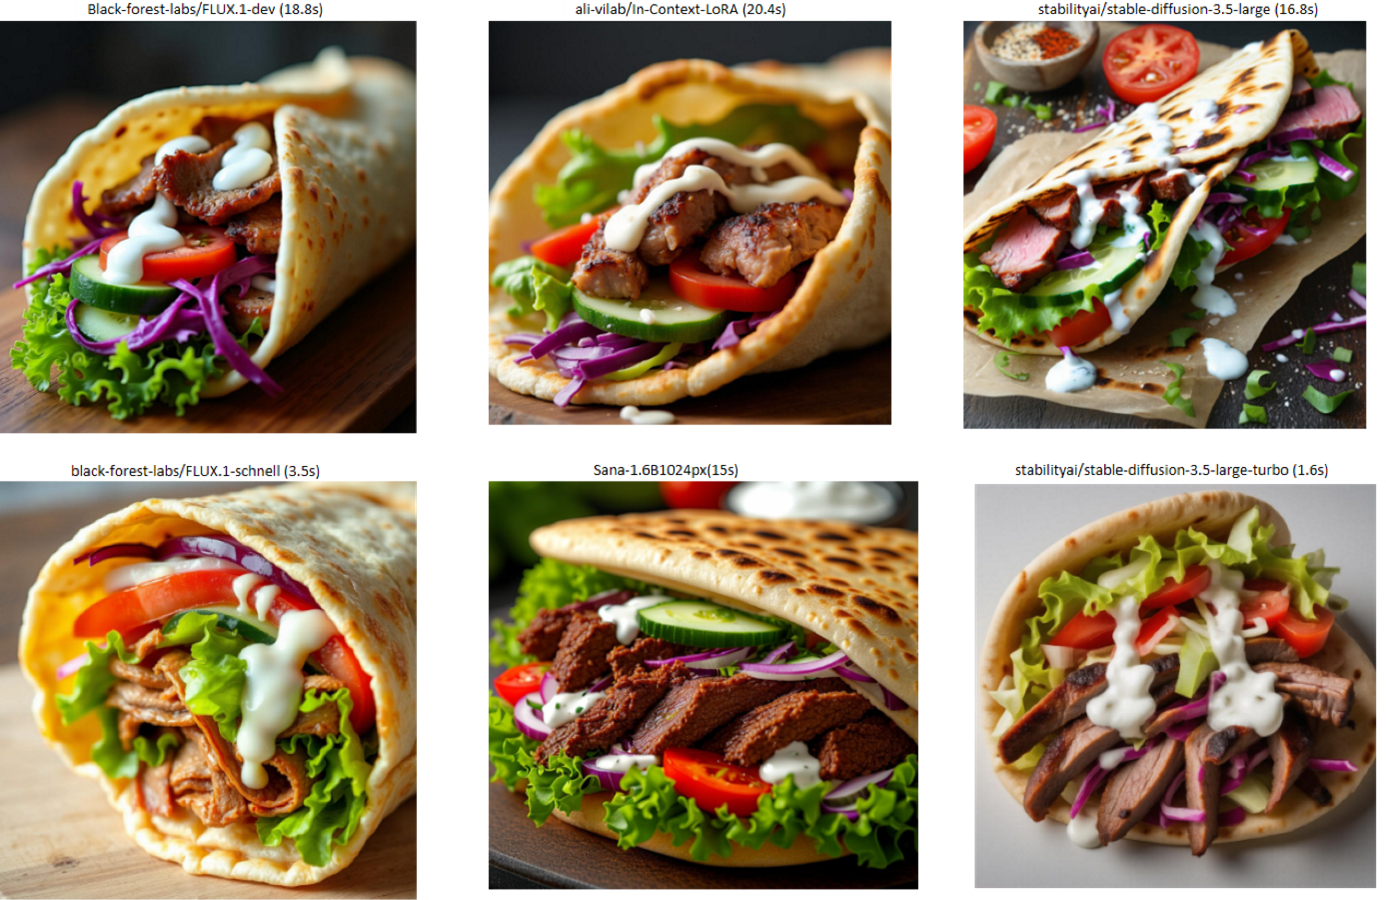
\includegraphics[width=\textwidth]{abbildungen/Results_image_generation}
    \caption{Vergleich der generierten Bilddateien durch die Text-to-Image Modelle}
    \label{fig:results_image_generation}
    \raggedright Quelle: Eigene Darstellung
\end{figure}

Abbildung \ref{fig:results_image_generation} zeigt eine Zusammenfassung der generierten Inhalte in der Kategorie Text-to-Image.
Positiv zu bewerten ist, dass alle der getesteten Modelle den Auftrag korrekt interpretiert haben und eine Detailaufnahme des geforderten Produktes erzeugt haben.
Unterschiede gibt es jedoch im erreichten Realismus der Produktbilder.
Die FLUX Modelle erzeugten hierbei die qualitativ hochwertigsten und realistischsten Bilder, die kaum von realen Produktbildern zu unterscheiden sind.
Die Stable Diffusion Modelle waren ebenfalls dazu fähig, inhaltlich korrekte, aber dennoch minderwertige Produktbilder zu generieren.
Bei näherer Betrachtung der abgebildeten Zutaten eine gewisse Künstlichkeit auf, die Rückschlüsse auf \ac{KI} generierte Inhalte schließen lässt.
Zudem erzeugen die Produktbilder nur mäßiges Interesse am Produkt, aufgrund der vergleichsweisen schlechten Komposition und stilistischen Umsetzung des Bildes.
Das \textit{Sana-\_1600M\_1024px} Modell erzeugte ein ähnlich gelungenes, visuell ansprechendes Produktbild, wie die Modelle \textit{FLUX.1-dev} und \textit{FLUX.1-schnell}, dennoch ist der Realismusgrad deutlich schlechter, da sich die Strukturen der abgebildeten Zutaten leicht von den Originalen unterscheiden.

\clearpage
\begin{figure}[htbp]
    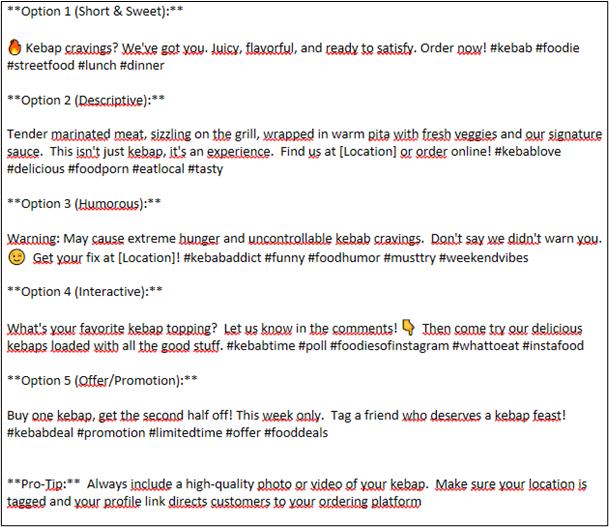
\includegraphics[width=\textwidth, height=\textheight, keepaspectratio]{abbildungen/textresult_gemini}
    \caption{generierter Text durch das Text-to-Text Modell gemini-1.5-pro}
    \label{fig:textresult_gemini}
    \raggedright Quelle: Eigene Darstellung
\end{figure}
Abbildung \ref{fig:textresult_gemini} zeigt exemplarisch die mit dem Text-to-Text Modell \textit{gemini-1.5-pro}, für Werbezwecke nutzbaren, Bildbeschreibungen.
Vergleicht man die Ergebnisse aller untersuchten Modelle miteinander, ist der über alle Modelle hinweg erreichte Realismusgrad positiv zu bewerten.
Jedes der getesteten Modelle erzeugte kurze, aussagekräftige, bildhafte und mit Schlagwörtern gefüllte Texte und baute zudem themenspezifische Hashtags ein.
Keine der generierten Bildbeschreibungen unterscheidet sich stark in Form und Inhalt von heutzutage gängigen Werbebeiträgen in sozialen Medien.
Hierbei auffällig ist, dass sowohl das \textit{QwQ-32B-Preview} Modell, als auch das \textit{Llama-3.1-Nemotron-70B-Instruct-HF} standardmäßig keine Emojis als stilistisches Mittel in den generierten Texten verwenden.
Darüber hinaus ist zu beobachten, dass das \textit{Llama-3.1-Nemotron-70B-Instruct-HF} fiktive Rabattaktionen bewirbt, dessen Generierung nicht durch Eingabeprompt gefordert waren.
Alle der untersuchten Text-to-Text Modelle, ausgenommen dem \textit{Mistral-7B-Instruct-v0.3} Modell, generierten zudem mehr als eine Bildbeschreibung, obwohl dies ebenfalls nicht im Eingabeprompt verlangt wurde.\footnote{Siehe Anhang, Abbildung \ref{fig:textresult_mistral},\ref{fig:textresult_Qwen},\ref{fig:textresult_nvdia_nemotron}.}

\begin{table}[h]
  \begin{tabular}{|p{3cm}|p{3cm}|p{2cm}|p{2cm}|p{3cm}|}
      \hline
      \textbf{Modellname} & \textbf{Modellziel} & \textbf{Modellgröße} & \textbf{Generierungsdauer} & \textbf{Qualität}\\ \hline
      {Black-forest-labs/FLUX.1-dev} & Text-to-Image & 23.8 GB & 18.8s & sehr gut\\ \hline
      {Black-forest-labs/FLUX.1-schnell} & Text-to-Image & 23.8 GB & \textless 5s & sehr gut\\ \hline
      {Efficient-Large-Model/Sana-\_1600M\_1024px} & Text-to-Image & 6.43 GB & \textless 5s & gut\\ \hline
      {Stabilityai/stable-diffusion-3.5-large} & Text-to-Image & 16.5 GB & 16.8s & befriedigend\\ \hline
      {Stabilityai/stable-diffusion-3.5-large-turbo} & Text-to-Image & 16.5 GB & 1.6s & ausreichend\\ \hline
      {Stabilityai/stable-diffusion-3.5-large} & Text-to-Image & 16.5 GB & 1.6s& befriedigend\\ \hline
      {Qwen/QwQ-32B-Preview} & Text-to-Text & \textgreater 50GB & 8s & sehr gut\\ \hline
      {gemini-1.5-pro} & Text-to-Text & \textgreater 100GB & 10s & sehr gut\\ \hline
      {mistralai/Mistral-7B-Instruct-v0.3} & Text-to-Text & 15.5 GB & \textgreater5s & sehr gut\\ \hline
  \end{tabular}
  \caption{Vergleich der generativen Machine Learning Modelle}\label{tab:table_modellvergleich}
  \raggedright Quelle: Eigene Darstellung
\end{table}

Tabelle \ref{tab:table_modellvergleich} zeigt eine Zusammenfassung der erfassten Kennzahlen über alle untersuchten Modelle.
Auffällig ist, dass die untersuchten Modelle mit dem Modellziel Text-to-Text, trotz ihrer unterschiedlichen Größe und Trainingsdaten, in der Generierungsdauer und Qualität der Ergebnisse kaum voneinander abweichen.
Die Modellgröße unterscheidet sich jedoch erheblich, wobei das \textit{Gemini-1.5-pro} Modell mit über 100GB das größte Modell, und das \textit{Mistral-7B-Instruct-v0.3} mit 15.5GB das kleinste Modell darstellt.
Aus Effizienzgründen ist das \textit{Mistral-7B-Instruct-v0.3} Modell für die Kategorie Text-to-Text, welches die qualitativ hochwertigsten Ergebnisse in kürzester Zeit generierte, zu bevorzugen.

Die untersuchten Modelle in der Kategorie Text-to-Image hingegen, zeigen deutliche Unterschiede in der Qualität der generierten Inhalte, wobei die FLUX Modelle die qualitativ hochwertigsten Ergebnisse erzielen.
Im direkten Vergleich erzielte hierbei das \textit{FLUX.1-schnell} Modell die besten Ergebnisse, da es die qualitativ hochwertigsten Bilder in kürzester Zeit generierte und somit zu bevorzugen ist.
\clearpage

\subsection{Auswahlprozess Web-Technologien}
Um geeignete Technologien für die Entwicklung der Applikation zu finden, wird ein Auswahlprozess durchgeführt.

Dieser Prozess folgt dem Konzept der \ac{PAPRIKA} Methode von Hansen und Ombler.
Zu Beginn wird eine Liste von Kriterien erstellt, die für die Auswahl der Technologien relevant sind.
Anschließend wird eine Gewichtung der Kriterien vorgenommen, um die Relevanz der einzelnen Kriterien zu bestimmen.
Nachdem die Kriterien festgelegt sind, werden die zu vergleichenden Technologien identifiziert.
Abschließend erfolgt die Bewertung der Technologien anhand der Kriterien, indem diese paarweise miteinander verglichen werden.
Dadurch wird für jede benötigte Komponente die am besten geeignete Technologie identifiziert.\footcite{Paprika2008}

Folgende Anforderungen wurden zur Bewertung der einzelnen Technologien identifiziert:

\begin{table}[htbp]
  \centering
  \begin{tabular}{|p{2cm}|c|p{5cm}|p{4cm}|}
      \hline
      \textbf{Kriterium} & \textbf{Gewicht} & \textbf{Beschreibung} & \textbf{Skala}\\ \hline
      {Lernkurve} & 0.4 & Lernaufwand in Relation zum Erfolgsgrad im Hinblick auf umzusetzende Features & flach, moderat, steil\\ \hline
      {Community} & 0.3 & Größe und Aktivität der Community sowie vorhandenes Lernmaterial & klein, mittel, groß\\ \hline
      {Bibliotheken} & 0.2 & Verfügbarkeit von Bibliotheken & begrenzt, mittel, umfangreich\\ \hline
      {Relevanz} & 0.1 & Aktualität und Weiterentwicklung der Technologie & niedrig, mittel, hoch\\ \hline
  \end{tabular}
  \caption{Bewertung der Anforderungen an Web-Technologien}\label{tab:table}
  \raggedright Quelle: Eigene Darstellung
\end{table}

Im nächsten Schritt werden die zu vergleichenden Technologien identifiziert.
Folgende Komponenten werden für die Entwicklung der Applikation benötigt:

\begin{itemize}
  \item Frontend-Framework
  \item Backend-Framework
  \item Datenbank
\end{itemize}

Um den Auswahlprozess zu vereinfachen, wird die Auswahl auf drei Technologien je Kategorie beschränkt.
Dabei erfolgt die Auswahl anhand von bereits vorhandenem Wissen und Erfahrungswerten.
Es wurden folgende Technologien für die Auswahl identifiziert:

\begin{table}[htbp]
  \centering
  \begin{tabular}{|l|c|c|c|}
      \hline
      \textbf{Technologie Kategorie} & \textbf{Top 1} & \textbf{Top 2} & \textbf{Top 3} \\ \hline
      {Frontend-Framework} & Angular & VueJS & React \\ \hline
      {Backend-Framework} & Flask & Django & Cherrypy \\ \hline
      {Datenbank} & PostgreSQL & MySQL & MongoDB \\ \hline
  \end{tabular}
  \caption{Technologieauswahl Übersicht}\label{tab:Technologieauswahl Übersicht}
  \raggedright Quelle: Eigene Darstellung
\end{table}

Zur Bestimmung der einzelnen Werte werden unterschiedliche Datenquellen herangezogen.
Zur Überprüfung der Relevanz wird die aktuelle Stackoverflow Developer Survey 2024\footcite{StackOverflow2024}, sowie State of JS 2023\footcite{stateofjsStateJavaScript2023} herangezogen.

Zusätzlich werden die Plattformen Github.com und Stackoverflow.com untersucht, inwiefern die Technologien dort vertreten sind.
Für die Frontend Frameworks im Speziellen werden die verfügbaren Libraries im Node Package Manager (NPM) untersucht.

Zur Bestimmung des Erscheinungsjahres der Technologien werden die offiziellen Dokumentationen bzw. die ersten Commits in den Repositories auf Github.com herangezogen.
Daraus ergeben sich folgende Quellen:
\begin{enumerate}
    \item Angular - Github Release\footcite{githubAngularReleaseV090}
    \item VueJS - Podcast mit Entwickler von VueJS\footcite{eggheadEvanYou}
    \item React - Github Changelog\footcite{githubReactCHANGELOG}
    \item Flask - PyPi Release\footcite{pypiFlask}
    \item Django - PyPi Release\footcite{pypiDjango}
    \item Cherrypy - PyPi Release\footcite{pypiCherryPy}
    \item PostgreSQL - Offizieller Blogpost von PostgreSQL\footcite{postgresqlHappyBirthday}
    \item MySQL - Amazon AWS Artikel\footcite{amazonWhatMySQL}
    \item Mongodb - Offizieller MongoDB Artikel\footcite{mongodbMongoDBEvolved}
\end{enumerate}

\newpage
Aus der vorangegangenen Analyse lassen sich folgende Daten ableiten:

\begin{table}[h!]
    \centering
    \begin{tabular}{|l|p{2cm}|p{3cm}|p{3cm}|p{3cm}|}
        \hline
        \rowcolor{lightgray} Name & \textbf{Datum Veröffentlichung} & \textbf{Aktive Fragen auf Stackoverflow} & \textbf{Repositories auf Github mit Tag} & \textbf{Abhängigkeiten NPM} \\ \hline
        Angular & 2010 & 306.845 & 57.588 & 14.607 \\ \hline
        VueJS & 2014 & 108.341 & 26.600 & 80.824 \\ \hline
        React & 2013 & 481.823 & 173.000 & 240.000 \\ \hline
        \hline
        Flask & 2010 & 55.856 & 50.985 & - \\ \hline
        Django & 2005 & 313.041 & 67.366 & - \\ \hline
        Cherrypy & 2004 & 1.370 & 147 & - \\ \hline
        \hline
        PostgreSQL & 1996 & 178.607 & 56.562 & - \\ \hline
        MySQL & 1995 & 661.661 & 75.826 & - \\ \hline
        Mongodb & 2009 & 176.192 & 111.693 & - \\ \hline
    \end{tabular}
    \caption{Analyseergebnise Relevanz der Plattformen}\label{tab:Analyseergebnise Relevanz der Plattformen}
    \raggedright Quelle: Eigene Darstellung
\end{table}

Darüber hinaus können die Ergebnisse der Studie von Bielek et al. herangezogen werden, welche Aufschluss über die Performance der einzelnen Technologien geben.
Aus der Untersuchung geht hervor, dass VueJS das effizienteste Frontend-Framework ist, gleichzeitig die niedrigste Anzahl an benötigten Programmcodes aufweist.\footcite{Bielak_2022}

Diese Erkenntnisse werden in der Untersuchung von Lipski et al. bestätigt.
Darüber hinaus wird in dieser Studie beschrieben, dass VueJS besonders für Entwickler ohne bisherige Erfahrung in der Webentwicklung geeignet ist.\footcite{Lipski_2021}

Diese Erkenntnisse wirkt sich positiv auf Lernkurve, wie auch die Relevanz der Technologie aus.
Die Syntax von VueJS bricht komplexe Zusammenhänge in einfachere Teile herunter, wodurch die Einarbeitung in die Technologie erleichtert wird.
Dadurch können gleiche Funktionen einfacher und schneller implementiert werden.

Auf Basis der gesammelten Daten und geleisteten Recherchen lassen sich die Technologien wie folgt bewerten:

\begin{table}[h!]
    \centering
    \begin{tabular}{|l|l|c|c|c|c|}
        \hline
        \rowcolor{lightgray} \textbf{Technologie} & \textbf{Kategorie} & \textbf{Community} & \textbf{Lernkurve} & \textbf{Bibliotheken} & \textbf{Relevanz} \\ \hline
        Angular & Backend Framework & \cellcolor{green!70}3 & \cellcolor{red!70}1 & \cellcolor{green!70}3 & \cellcolor{orange!70}2 \\ \hline
        VueJS & Backend Framework & \cellcolor{green!70}3 & \cellcolor{green!70}3 & \cellcolor{orange!70}2 & \cellcolor{green!70}3 \\ \hline
        React & Backend Framework & \cellcolor{green!70}3 & \cellcolor{orange!70}2 & \cellcolor{green!70}3 & \cellcolor{green!70}3 \\ \hline
        Flask & Frontend Framework & \cellcolor{orange!70}2 & \cellcolor{green!70}3 & \cellcolor{orange!70}2 & \cellcolor{orange!70}2 \\ \hline
        Django & Frontend Framework & \cellcolor{green!70}3 & \cellcolor{red!70}1 & \cellcolor{green!70}3 & \cellcolor{green!70}3 \\ \hline
        Cherrypy & Frontend Framework & \cellcolor{red!70}1 & \cellcolor{orange!70}2 & \cellcolor{red!70}1 & \cellcolor{red!70}1 \\ \hline
        PostgreSQL & Datenbank & \cellcolor{green!70}3 & \cellcolor{orange!70}2 & \cellcolor{green!70}3 & \cellcolor{green!70}3 \\ \hline
        MySQL & Datenbank & \cellcolor{green!70}3 & \cellcolor{green!70}3 & \cellcolor{orange!70}2 & \cellcolor{orange!70}2 \\ \hline
        Mongodb & Datenbank & \cellcolor{green!70}3 & \cellcolor{orange!70}2 & \cellcolor{green!70}3 & \cellcolor{green!70}3 \\ \hline
    \end{tabular}
    \caption{Bewertung von Technologien}
    \label{tab:Tabelle Bewertung von Technologien}
    \raggedright Quelle: Eigene Darstellung
\end{table}

Zuletzt werden die jeweiligen Technologien paarweise miteinander verglichen.
Dabei wird die Bewertung der einzelnen Kriterien in Relation zueinander gesetzt, um die am besten geeignete Technologie zu identifizieren.
Neben den erhobenen Daten fließen auch subjektive Einschätzungen in die Bewertung mit ein.
\newpage
\textbf{Frontend-Framework:}

Angular und VueJS sind beide als Webtechnologie etabliert und weisen eine entsprechende Community auf.
Ebenso gibt es für beide Tools zahlreiche Communities, wobei sich Angular dort besonders hervortut.
Für die Relevanz der Technologien erscheint VueJS jedoch vielversprechender.
Der entscheidende Faktor in diesem Vergleich ist die Lernkurve der Technologien, bei welcher VueJS mit einer flachen Einstiegserfahrung überzeugt.%Todo: Quelle
Daher fiel die Entscheidung auf VueJS.

Beim Vergleich von Angular und React zeigt sich, dass React ebenfalls äußerst etabliert ist und als eines der beliebtesten Frontend-Frameworks gilt.%Todo: Quelle
Der Umfang an verfügbaren Bibliotheken ist mit Angular vergleichbar.
Jedoch ist die Lernkurve von React im Vergleich zu Angular einfacher, was zu einer Entscheidung zugunsten von React führte.%Todo: Quelle

Der Vergleich von VueJS und React zeigt, dass beide Technologien im Hinblick auf die Community gleichauf sind.%Todo: Quelle
Das Angebot an Bibliotheken ist für React dennoch größer.%Todo: Quelle
Beide Frameworks gelten als äußerst relevant für moderne Applikationen.%Todo: Quelle
Entscheidender Faktor im Vergleich ist die Lernkurve, bei welcher VueJS mit einer flachen Einstiegserfahrung überzeugt.%Todo: Quelle
Aus diesem Grund fiel die Wahl erneut auf VueJS.

In der gesamten Betrachtung der Frontend-Frameworks ist VueJS die Technologie, die am besten zu den Anforderungen passt.

\newpage
\textbf{Backend-Framework:}
Flask und Django stellen die beiden beliebtesten Python-Frameworks zur Entwicklung von Webapplikationen dar, wobei Django die größere Community aufweist.%Todo: Quelle
Daraus resultiert ein größeres Angebot an Bibliotheken für Django im Vergleich zu Flask.%Todo: Quelle
Ebenso die Relevanz der Technologie ist für Django höher einzustufen.%Todo: Quelle
Über die Lernkurve lässt sich sagen, dass Flask eine flachere Lernkurve aufweist als Django, welches eher als steil zu bewerten ist.%Todo: Quelle
Im direkten Vergleich ist jedoch der Lernaufwand für Django gerechtfertigt, da die Technologie eine Vielzahl an Features bietet und durch die große Community und dem Angebot an Bibliotheken unterstützt wird.
Dadurch ist die Entscheidung auf Django gefallen.

Der Vergleich von Flask und Cherrypy zeigt, dass Flask in allen betrachteten Kriterien besser abschneidet.
Die Community ist größer, das Angebot an Bibliotheken umfangreicher und die Relevanz höher einzustufen.%Todo: Quelle
Auch die Lernkurve wird flacher gewertet als bei Cherrypy, wodurch die Entscheidung, im direkten Vergleich, auf Flask fällt.%Todo: Quelle

Django ist, ebenso wie Flask, in fast allen Kriterien besser zu bewerten als Cherrypy.
Einzig die Lernkurve ist bei Cherrypy flacher einzustufen.
Dennoch überzeugt Django durch die größere Community, das umfangreichere Angebot an Bibliotheken und die höhere Relevanz, weswegen die Entscheidung auf Django fällt.%Todo: Quelle

In der gesamten Betrachtung der Backend-Frameworks ist Django die Technologie, die am besten zu den Anforderungen passt.

\textbf{Datenbanken:}

PostgreSQL und MySQL sind beide als relationale Datenbanken etabliert und weisen eine entsprechende Community auf.
Dabei gilt MySQL als die einsteigerfreundlichere Datenbank während PostgreSQL eine weitere Verbreitung in der gegenwärtigen Technologielandschaft aufweist.%Todo: Quelle
Zudem gilt PostGreSQL als die relevantere Technologie.%Todo: Quelle
Aufgrund der zuvor abgestimmten Gewichtung der Kriterien fällt die Entscheidung auf MySQL.

Der Vergleich von PostgreSQL und MongoDB zeigt, dass die betrachteten Merkmale in etwa gleich zu bewerten sind.
Zentraler Unterschied zwischen beiden Technologien ist die Art der Datenbank, wobei PostgreSQL als relationale Datenbank und MongoDB als NoSQL-Datenbank klassifiziert wird.%Todo: Quelle

Für die Entscheidung über die Datenbanktechnologie wird PostgreSQL als SQL bzw. MongoDB als NoSQL Variante gewählt.
Im Rahmen der Architekturkonzipierung können beide Technologien in Betracht gezogen werden, wobei die Entscheidung auf Basis der spezifischen Anforderungen der Applikation getroffen wird.



